%%%%%%%%%%%%%%%%%%%%%%%%%%%%%%%%%%%%%%%%%
% FRI Data Science_report LaTeX Template
% Version 1.0 (28/1/2020)
% 
% Jure Demšar (jure.demsar@fri.uni-lj.si)
%
% Based on MicromouseSymp article template by:
% Mathias Legrand (legrand.mathias@gmail.com) 
% With extensive modifications by:
% Antonio Valente (antonio.luis.valente@gmail.com)
%
% License:
% CC BY-NC-SA 3.0 (http://creativecommons.org/licenses/by-nc-sa/3.0/)
%
%%%%%%%%%%%%%%%%%%%%%%%%%%%%%%%%%%%%%%%%%


%----------------------------------------------------------------------------------------
%	PACKAGES AND OTHER DOCUMENT CONFIGURATIONS
%----------------------------------------------------------------------------------------
\documentclass[fleqn,moreauthors,10pt]{ds_report}
\usepackage[english]{babel}
\usepackage{graphicx}
\usepackage{supertabular}
\usepackage{multicol}
\usepackage{caption}
\usepackage{graphicx}
\usepackage{subcaption}
\usepackage{float}
\usepackage{hyperref}

\graphicspath{{fig/}}

%----------------------------------------------------------------------------------------
%	ARTICLE INFORMATION
%----------------------------------------------------------------------------------------

% Header
\JournalInfo{Paraphrasing sentences}

% Interim or final report
\Archive{Project report} 
%\Archive{Final report} 

% Article title
\PaperTitle{Paraphrasing sentences} 

% Authors (student competitors) and their info
\Authors{Aljaž Grdadolnik, Anže Mihevc, and Luka Galjot}

% Advisors
\affiliation{\textit{Advisors: Slavko Žitnik}}

% Keywords
\Keywords{Transformer-Based Language Models, T5, paraphrasing, Transformer-Based Language Models}
\newcommand{\keywordname}{Keywords}


%----------------------------------------------------------------------------------------
%	ABSTRACT
%----------------------------------------------------------------------------------------

\Abstract{
This report discusses the use of deep learning models, particularly transformer-based language models like T5, to implement sentence paraphrasing, which is a crucial aspect of natural language processing tasks. The aim is to use a fine-tuned version of T5 to generate paraphrases of sentences by selecting a corpus that includes semantically similar paraphrases while preserving the original meaning. The paper proposes to validate the model using both manual and automatic metrics. The implementation of this approach has the potential to improve the efficiency of natural language processing tasks.
}

%----------------------------------------------------------------------------------------

\begin{document}

% Makes all text pages the same height
\flushbottom 

% Print the title and abstract box
\maketitle 

% Removes page numbering from the first page
\thispagestyle{empty} 

%----------------------------------------------------------------------------------------
%	ARTICLE CONTENTS
%----------------------------------------------------------------------------------------

\section*{Introduction}

Paraphrasing, the process of expressing the same meaning using different words is an important part of natural language processing tasks. Recently, deep learning models, particularly the transformer-based language models like BERT, have achieved remarkable results in several language processing tasks. This paper aims to implement sentence paraphrasing using T5 Text-to-Text Transfer Transformer model, which has demonstrated state-of-the-art performance in range of processing tasks. Specifically we will use fine-tuned version of T5 \cite{ulčar2023sequence} to generate paraphrases of sentences. Fine-tuning will be performed by one of the selected corpora, which will be preprocessed to include semantically similar paraphrases while preserving the meaning of the original sentence. We will validate our model with manually defined metrics and automatic methods. 

%------------------------------------------------

\section*{Related work and existing solutions}
Recently with emergence of ChatGPT service many of other companies and academic groups have speed up development of their own LLMs such as GPT-2 (by OpenAI), GPT-3 (by OpenAI), T5 (by Raffel et al. \cite{https://doi.org/10.48550/arxiv.1910.10683}), RoBERTa (by Liu et al. \cite{https://doi.org/10.48550/arxiv.1907.11692}), LLaMa (by Touvron et al. \cite{https://doi.org/10.48550/arxiv.2302.13971}).

In the article \textit{\textbf{The Multilingual Paraphrase Database}}\cite{ganitkevitch2014multilingual} the authors expand their English and Spanish paraphrase database to include 21 other languages including Slovene. They extract the paraphrases from bilingual parallel corpora by “pivoting” words and phrases over a shared translation in another language (English). They make the database freely available. 



%------------------------------------------------

\section*{Initial ideas}
This section aims to provide initial ideas on how to approach the classroom project.

\subsection{Dataset acquisition/generation}
Perhaps the most important part of training a good model for paraphrasing is starting with the right dataset. The dataset should include quality pairs of phrases and their paraphrases. Such datasets already exist mainly for the English language such as The Paraphrase Database (PPDB)\cite{ganitkevitch2013ppdb}. We have found an extended version of PPDB that includes other languages including Slovene\cite{ganitkevitch2014multilingual}. Upon further investigation we have determined that the phrases included in this extended database are often only synonyms and the “source” phrases are not longer than 6 words. This dataset was produced using the back translation method or by “pivoting” over a shared translation in another language, in this case English. We would like to see if we get better results using a different method such as automatic translation of non-Slovene dataset. We will use a translation model provided in the instructions of this assignment \cite{Slovene_nmt} to automatically translate the original PPDB to Slovene. Afterwards we will check the quality and similarity of the translated pairs using different metrics. If our method produced better results than the back translation method we would use the automatically translated dataset to train our paraphrasing model.

More recently the QUORA\cite{sambit7_quora_dataset} and MSCOCO\cite{lin2014microsoft} dataset have been used to train and evaluate paraphrasing models. The QUORA dataset is a dataset of duplicate questions posted on the Quora website. This questions are manually marked by moderators as duplicates so they are confirmed paraphrases. We could use automatic translation to obtain paraphrasing pairs in Slovene. The MSCOCO dataset is not a dataset originally made for paraphrasing or language processing rather it is a dataset of objects and object recognition within images. However the dataset specifically the annotations of the images can still be used to train and test paraphrasing models. To use this model in our assignment we would again need to automatically translate it and check for the quality of the translated pairs.

\subsection{Natural language deep learning model}
To implement paraphrasing, we can use a deep learning model to fine-tune T5 model on pairs of sentences. The T5 model is a transformer-based model that is pre-trained on a large corpus of text. Fine-tuning the T5 model on pairs of sentences will allow us to train the model to generate paraphrases of the input sentences. The deep learning model will learn to generate paraphrases by minimizing the difference between the predicted paraphrase and the actual paraphrase. This approach has been shown to be effective in generating high-quality paraphrases.

\subsection{Result evaluation}
The quality of the implemented model has to be somehow evaluated so we can compare it to other already existing models. For this we will use different metrics of evaluation. These are BLEU (\textit{Bilingual Evaluation Understudy)} which was developed to evaluate machine translation systems, but can be also used for paragraph evaluation, METEOR(\textit{Machine Translation Evaluation Overlap Rate}) which aims to address BLEU's weakness of being unable to measure semantic equivalents when applied to low-resource languages and has a better correlation with human judgement at the sentence/segment level than BLEU(\textit{Google-BLEU}), GLEU, ROUGE(\textit{Recall-Oriented Understudy for Gisting Evaluation}) a recall-based evaluation metric originally developed for text summarization, has also been used to evaluate paraphrase generation, BERTscore that is based on contextual embeddings from BERT and cosine similarity between the generated sentence and one or more reference sentences and WER(\textit{Word Error Rate}), which is a metric that measures the similarity between two sentences by counting the number of word insertions, deletions and substitutions needed to transform one sentence into another\cite{zhou2021paraphrase}. And lastly we will use human evaluation as a metric, which will probably be the best in scoring, but most definitely the most tedious and time consuming.

\section{Datasets}

% TODO 
%- mal o teh datasetih k smo jih prej predlagal zakaj se nismo pol odločl za njih
%- MaCoCu dataset zakaj sm ose za tega odloč, kako je strukturiran, kako smo ga mi prpravl, kako smo ga prevedl, kako smo ga pol pretvorl v csv in kako smo ga dal na Huggingface

\subsection{Proposed datasets}
We searched for datasets from different resources, such as clarin\cite{Clarin}, Corpus\cite{opensubtitles} \cite{TIEDEMANN12.463} and the shared repository for corpora where teams could upload their own corpora.

\subsubsection{OpenSubtitles}
\label{sub-sec:open-sub}
% TODO kaj smo probal pa zakaj ni šlo
%- mal o podnapisih zakaj ni šlo itd. 
For the subtitles we chose to use the Opus\cite{opensubtitles} \cite{TIEDEMANN12.463} dataset, which contains 65 languages and 2,793,243 files. We use the English and Slovene files, where there were approximately 20,000,000 parallel sentences. We had three files where ones was the English sentences, each of them in a separate line, the same was with the Slovene sentences and also a file for ids, which described where in the line each segment is since a sentence can have multiple segments. We ignored the last file and took a whole sentence as a segment.

Firstly we translated the English sentences into Slovene(with a help of group \emph{Skupina-8}) and then pre-processed the sentences as described in the \nameref{sub-sec:preprocess}.
%We removed the files that contained any weird characters such as (,),$<$,$>$, any incorrectly encoded characters such as \emph{č},\emph{š},\emph{ž}, we also removed hyphens with a space on each side, which there were many in the dataset, we also removed short sentences. This in the end left us with approximately 3 million sentences. We further pruned the dataset with calculating the ROUGE score on it and removed any paraphrases which had a score higher than 0.8. We also tried with paraphrases that had score of less than 0.6 and 0.1 so that we could see if that would give us an even better result, but we found out that bot 0.6 and 0.1 gave us worst results. The last thing we did was to remove the duplicated sentences, which there were many. In the end we were left with one and a half million sentences.

\subsubsection{MaCoCu}
For the corpus in this part of the project we used \emph{Slovene web corpus MaCoCu-sl 1.0
} which was built by crawling the \emph{.si} internet domain in 2021. The corpus is made of 3176311 sentences in both English and Slovene.

The corpus contains one file where in each line there is an English sentence and it's Slovene counterpart separated by a tab.

We then translated (with a help of nlp-course-skupina-8) the English part to Slovene and made a new file which consists of two similar Slovene sentences separated with a tab. After translation there were 2884462 sentences left, because in the translation we pruned some of the sentences if they were too short or had too many special characters or numbers. Once that was done, we uploaded the corpus on a \emph{sharepoint} link and on \emph{hugging face}(but only a corpus of 250 thousand sentences, these are the same we trained our model on) in repository \emph{hieronymusa/MaCoCu-dataset-250k} with three files stored in folder called data. The three files are train, validation and test csv file. These and the one on \emph{sharepoint} can be used by any other group. We can add that there was an update to the \emph{Slovene web corpus MaCoCu-sl 1.0} called \emph{Slovene web corpus MaCoCu-sl 2.0
} uploaded just one day after we translated the version one.

Once we had the original Slovenian sentences and the translated sentences we had to pre-process the data so that we could use it to fine tune our model. We wrote a short python script that creates one csv file from the files with original and translated sentences. Each line in the generated csv file consists of 3 columns: ID, Original and Translated[Paraphrased]. ID column is simply the sequential number of the line, the Original column is the original Slovenian sentence and the Translated[Paraphrased] is the the translated Slovenian sentence. 
The script can create sub-sets of the dataset starting and finishing the subset at arbitrary points in the dataset. We used the script to create smaller sub-sets of the dataset to enable us to train the model faster. 
This greatly reduces the quality of the results but enables us to check the influence of different parameters such as batch size and number of epochs on the training time. Once we found the optimal parameters we used the entire dataset to train our model. 

\subsection{Preprocesing the data}
\label{sub-sec:preprocess}
After training the model with the full MaCoCu dataset we realized that some input data was already a bad representation of a paraphrase. These sentence pairs only had small changes between Original and the Translated sentence.   

We removed the sentence pairs that contained any weird characters such as (,),$<$,$>$, any incorrectly encoded characters such as \emph{č},\emph{š},\emph{ž}, we also removed hyphens with a space on each side, which there were many in the dataset, we also removed short sentences. We further pruned the dataset with calculating the ROUGE score on sentence pairs and removed any that had a score higher than 0.8. We also tried with pairs that had score of less than 0.6 and 0.1 so that we could see if that would give us an even better result, but we found out that bot 0.6 and 0.1 gave us a worst results. The last thing we did was to remove the duplicated sentences, which again there were many. In the end we were left with one and a half million sentences.

We pre-processed the OpenSubtitles dataset in the same way.


\section{Models}

We discovered that the sloBerta model would not work for our task as it is not a generative model. We looked at the generative models that would be better suited for our task and decided to use the T5 model. More specifically the T5-sl model which is already capable of producing Slovene text. For the initial stage we will be using the \emph{t5-sl-small} version of the model as we want relatively fast iterations so we can test our code and different parameters. This model has 8 encoder and 8 decoder layers with total of about 60 million parameters and was trained for five epochs on the corpora:
\begin{itemize}[itemsep=2pt]
    \item Gigafida 2.0,
    \item Kas 1.0,
    \item Janes 1.0,
    \item Slovenian parliamentary corpus siParl 2.0,
    \item slWaC
\end{itemize}

Even with this smaller model our home computers take a long time to fine tune the model. Thus we decided to run the training of our model on the ARNES cluster. Here we set up a singularity container using a Pytorch docker image as a base and installing some additional required packages. We ran into some problems when creating the images as each user only has 20GB of disk space allocated on his home directory. This was solved by saving the container elsewhere on the cluster. 

\subsection{Code and training the model}
The code we used for training our model is available on our GitHub~\cite{GitHub}. We first load our model \emph{t5-sl-small} then load the dataset from a local .csv file. We experimented with creating and uploading our own dataset to Huggingface website which we were able to do for the 250k long sub-set of our dataset. To have more granular and dynamic control over the data we use we still load the data from a local file but in the future we might upload the entire dataset to the Huggingface website and load the data from there.

After the data is loaded we initialize our metrics and tokenizer. Before we can use the data to train our model we have to add the prefix "paraphrase" to our original sentences so the model will learn what to do when it encounters the prefix. In the final version of fine-tuning the model we used the following values for the arguments (here only the interesting arguments are shown to see all the argument check our code on GitHub~\cite{GitHub}): 

\begin{itemize}[itemsep=2pt]
    \item learning\_rate=3e-5,
    \item num\_train\_epochs=3,
    \item per\_device\_train\_batch\_size=24
\end{itemize}

When the training is complete we save the model to a directory. 

To generate outputs using our model we can load our model from the directory in which we previously saved it. Then we provide the model with our input sentence which must start with the same prefix that we used in training the dataset. We use a tokenizer to tokenize the input and pass it to our model which generates a prediction. We then decode the prediction and print it out. 

In the end we fine-tuned a few different models using this same process. Depending on the size of the dataset the fine-tuning took from 40min to 10+ hours. We also had some difficulty getting the necessary resources on the ARNES supercomputer cluster as other users also ran long and demanding jobs. Some of our fine-tuning runs even failed due to different errors but the most prevalent one was running out of allocated disk space on the cluster. Here is a list of the fine-tuned models we were able to successfully train: 
\begin{itemize}
    \item t5-sl-small fine-tuned with 250k pairs from MaCoCu dataset (1 epoch)
    \item t5-sl-small fine-tuned with filter MaCoCu dataset (3 epochs)
    \item t5-sl-small fine-tuned with combined and filtered MaCoCu and OpenSubtitles dataset (3 epochs)
    \item some other smaller test t5-sl-small models
\end{itemize}

\section{Results}
\label{sec:results}
\subsection{Trained with smaller dataset (250k pairs)}
Because we use only a small sub-set of the dataset and a low number(1) of epochs the model returns the same sentence as the input most of the time. It does sometimes correct small grammatical errors and in some cases changes a word. We can see some examples bellow and even more examples in the \nameref{sec:appendix}.

\begin{itemize}
\item \emph{Same sentence as input:}
\item \textbf{Input}: paraphrase: Danes je lep dan 
\item \textbf{Output}: Danes je lep dan
\item \textbf{Input}: paraphrase: S tem bomo preprečili onesnaževanje narave in ohranjali zdravo okolje. 
\item \textbf{Output}: S tem bomo preprečili onesnaževanje narave in ohranjali zdravo okolje.
\item \emph{Grammatical correction:}
\item \textbf{Input}: paraphrase: Danes sem šel v trgovin in kupil kruh, mleko in jajca. 
\item \textbf{Output}: Danes sem šel v trgovino in kupil kruh, mleko in jajca.
\item \textbf{Input}: paraphrase: Ta denar nisem ukradel. 
\item \textbf{Output}: Ta denar sem ukradel.
\end{itemize}

The model performs better on longer sentences which makes sense as there are more words it can potentially swap or change. 

\subsection{Trained with the whole MaCoCu dataset}

After playing around with the models, consulting with the assistants and other teams we determined that the parameters used when generating outputs have a larger impact on the generated paraphrases than was previously considered. We wanted to optimize this parameters to get better results from our model. We found that what made the biggest difference in generated output was using or not using the parameter num\_beams. When setting this parameter we would only get minor changes in the generated paraphrases compared to the original sentence. But when not using the parameter the model would often generate sentences that are "very far" from the original sentence and sometimes completely unrelated sentences would be generated. We tested a lot of different combinations of parameters but even so there is a possibility that we missed some combination that would have worked better.\\

We determined that the best parameters for our model were: 
\begin{itemize}
    \item num\_beams=4
    \item num\_beam\_groups=notset
    \item do\_sample=True
    \item num\_return\_sentences=5
\end{itemize}

The combination of this parameters means that the model is using \textit{beam-search multinomial sampling} to generate the output. This is a combination of 2 techniques used in natural language processing tasks. Beam search is a heuristic search algorithm that is commonly used in sequence generation tasks. In the context of natural language processing, it is often employed to generate the most likely sequence of words given a particular model. Beam search focuses on a fixed number of the most promising candidates at each step of the generation process instead of exhaustively exploring all possible sequences. Multinomial sampling is a probabilistic technique used to sample from a multinomial distribution. In the context of natural language processing, it is often used to introduce randomness and diversity into the generated text. Instead of always selecting the most likely word according to the model's probability distribution, multinomial sampling allows for the possibility of sampling less likely words as well. Combining beam search with multinomial sampling involves using beam search to maintain a set of candidate sequences and then applying multinomial sampling to select the next word from the probability distribution at each step. This combination helps to generate more diverse and contextually relevant sequences by considering a range of likely candidates while introducing randomness into the selection process.\\

In addition we looked at all of the generated samples and discarded the ones that looked exactly like the input sentence. We then returned one of this outputs as a paraphrase.

Even with this parameters our model only makes minor changes to the sentence and only occasionally produces a good paraphrase. More on this in section titled \nameref{sec:eval}. It does however often combine two sentences into one while keeping the sentence semantically and grammatically correct. It also often fixes any grammatical errors in the original sentence and places commas in the correct places.\\

Examples of generated sentences can be found in section bellow titled \nameref{sec:eval}, in the \nameref{sec:appendix} and on our GitHub~\cite{GitHub}.

\section{Evaluation}
\label{sec:eval}

For evaluation we generated 88 sentence pairs. The original sentences were taken from a dataset that other teams uploaded on the OneDrive provided by the course. More specifically we took 88 sentences from the \textit{Sentence paraphrasing (Team 2357)/translated ccgigafida} dataset. The paraphrases were generated using our models and the parameters described in the section ~\nameref{sec:results}. We used this generated pairs to run our automatic and manual evaluation. 

\subsection{Automatic evaluation}
We used the the following metrics:
\begin{itemize}[itemsep=2pt,parsep=2pt,topsep=2pt]
    \item BLEU\cite{HuggingFaceMetrics}
    \item ROUGE1\cite{HuggingFaceMetrics}
    \item ROUGE2\cite{HuggingFaceMetrics}
    \item ROUGEL\cite{HuggingFaceMetrics}
    \item ROUGELSUM\cite{HuggingFaceMetrics}
    \item BERTScore F1\cite{HuggingFaceMetrics}
    \item BERTScore precision\cite{HuggingFaceMetrics}
    \item BERTScore recall\cite{HuggingFaceMetrics}
    \item WER\cite{HuggingFaceMetrics}
    \item METEOR\cite{HuggingFaceMetrics}
    \item GLEU\cite{HuggingFaceMetrics}
    \item ParaScore\cite{GitHubParaScore}
\end{itemize}
We only used BLEU on the whole dataset and got 0.17 as the result. For the dataset on which we did manual evaluation, which is described in the \nameref{sub-sec:manual_evaluation}, we evaluated it automatically with the before mentioned metrics. The results can be seen in the table \ref{tab:metrics-results}.

\begin{table}[h]
    \centering
    \scalebox{1}{
    \begin{tabular}{c|c}
       Metric name  & result \\
       \hline\hline
        BLEU & 0.73  \\
        ROUGE-1 & 0.88  \\
        ROUGE-2 & 0.78 \\
        ROUGE-L & 0.87 \\
        ROUGE-Lsum & 0.87 \\
        BERTScore F1 & 0.95 \\
        BERTScore precision & 0.95 \\
        BERTScore recall & 0.95 \\
        WER & 0.19 \\
        METEOR & 0.87 \\
        Google BLEU & 0.72 \\
        ParaScore & 0.92
    \end{tabular}
    }
    \caption{Results for different metrics on the 88 sentences.}
    \label{tab:metrics-results}
\end{table}

We can see that we got quite decent results, but as we can see in \nameref{sub-sec:manual_evaluation}, the automatic result are not close to the ones we get with manual evaluation. This can be due to a small dataset which was only 88 sentences that is due to a fact that we manually evaluated that many sentences and wanted to see a comparison between automatic and manual evaluation. For a better result we would have to have a bigger man power so we could manually evaluate a bigger dataset and also evaluate automatically a bigger dataset.

The thesis that the results are as good as they are because of the small dataset is the fact that the result for BLEU on the whole dataset of approximately two and a half million sentences is only 0.17 compared to 0.73 on the 88 sentences.

We expected a much lower score for ParaScore since it is the only metric here that was purposely designed for evaluation of paraphrases, but it should be also tested on a much larger evaluation dataset and compared to human evaluation.

\subsection{Manual evaluation}
\label{sub-sec:manual_evaluation}

For manual evaluation we propose three different "scores": 
\begin{itemize}
    \item \textit{\textbf{Changed words}}: is the total number of words/changes in the paraphrase compared to the original sentence.
    \item \textit{\textbf{Semantic correctness}}: a score from 0 to 2 where; 0 means the sentence has completely different meaning than the original, 1 means it is mostly the same and 2 is completely the same. 
    \item \textit{\textbf{"Intuition"}}: a score of "better"(2), "equal"(1) and "worse"(0). A paraphrase is  better/equal/worse compared to what a human would make. If a pair got 2 we would say that it is indistinguishable from a human made paraphrase. This is the most subjective of the scores.
\end{itemize}

We scored 20 pairs together as a team and then each member scored another ~20 sentences on their own. This gave as the scores for 88 sentence pairs. For an easier representation we summed up the scores in too one score caled Sum score. \\

We can see some of the results of the manual evaluation in the table~\ref{tab:manual_evaluation} in \nameref{sec:appendix}. In the table we can first see two examples of very bad paraphrases where the model changed the semantic meaning of the sentence too much. These kinds of sentence generally got a Sum score of 3 or lower. A bit better were pairs that got a Sum score of 4 or 5. We can see a representation of such sentences in the next two samples in the table. These sentences were semantically very similar to the original sentence, made some changes and usually got an intuition score of at least 1. The last two entries in the table represent very good paraphrases. These pairs were semantically the same, made a lot of changes and sometimes got an intuition score of 2. The whole table of our manual evaluation is available on our GitHub~\cite{GitHub}. The averages for each score can be seen in the bottom of the table. In general our model got quite low averages across all the scores but especially on the intuition score where it got an average of 0.55 (values 0-2). The average sum score indicates that our model is somewhere in-between not good and acceptable.

In conclusion, we can see that manual evaluation is still the best way to be sure that the paraphrases generated are sufficiently good, but because of lack of man power and also cost we can say that best automatic evaluation metrics are BLEU, WER and ParaScore.

\section{Conclusion}

In this project we used a T5 generative model and fine-tuned it with a dataset we created and preprocessed for paraphrasing sentences. Because this is computationally expensive we used the ARNES supercomputer cluster to train and use the models. We fine-tuned the model using different data-sets and evaluated them using automatic scores such as Rouge, Bleu, BertScore, Wer and Meteor. We also evaluated one of the models manually using scores we designed. We determined that even with automatic scores indicating good results our model did not preform well on the manual scores. Most of the paraphrases only had minor changes to the original sentence although there are some examples where the model made a very good and convincing paraphrases. Further improvement would be possible by using a bigger model such as the t5-sl-large. The dataset could also be improved as we noticed that our dataset does not include a lot of examples of first person sentences and thus our model is bad at paraphrasing such sentences. The output parameters could also be further optimized to generate better quality outputs.


%----------------------------------------------------------------------------------------
%	REFERENCE LIST
%----------------------------------------------------------------------------------------
\bibliographystyle{unsrt}
\bibliography{report}

\newpage
\onecolumn

\section{Appendix}
\label{sec:appendix}
\begin{figure}[H]
    \centering
    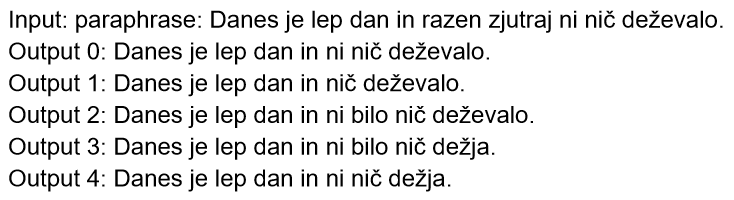
\includegraphics[width=0.33\columnwidth]{NLP_LaTeX_Template/fig/outputs/LepDan.png}
    \caption{Input and 5 different outputs of our model trained on 250K dataset. }
    \label{fig:output1}
\end{figure}

\begin{figure}[H]
    \centering
    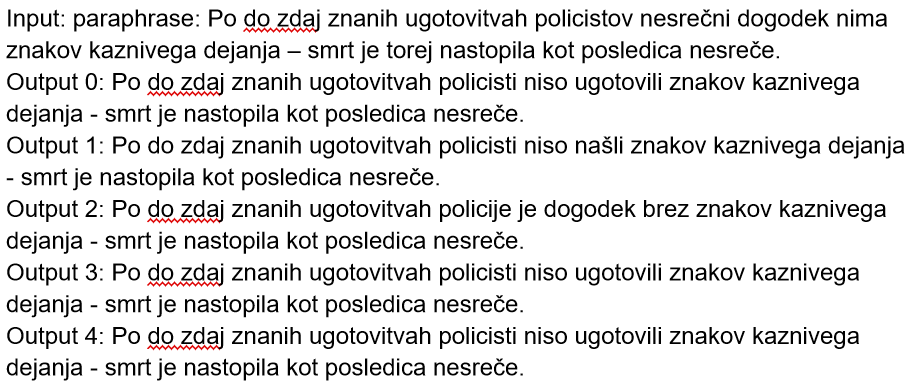
\includegraphics[width=0.4\columnwidth]{NLP_LaTeX_Template/fig/outputs/Obdukcija.png}
    \caption{Input and 5 different outputs of our model trained on 250K dataset. }
    \label{fig:output2}
\end{figure}


\begin{figure}[H]
    \centering
    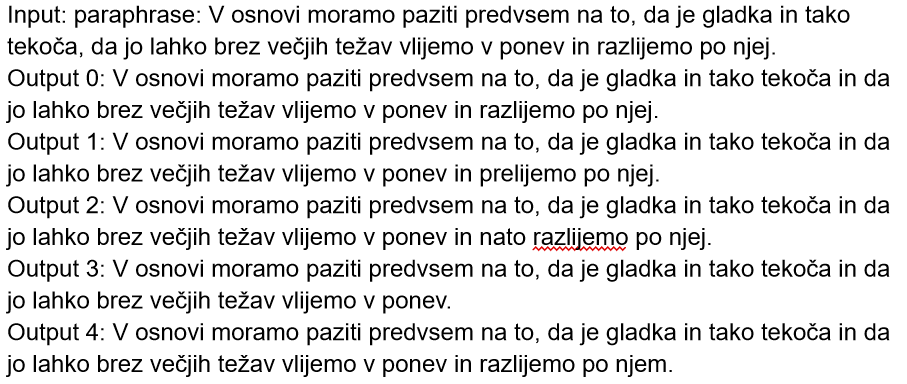
\includegraphics[width=0.4\columnwidth]{NLP_LaTeX_Template/fig/outputs/palačinke.png}
    \caption{Input and 5 different outputs of our model trained on 250K dataset. }
    \label{fig:output3}
\end{figure}


\begin{figure}[H]
    \centering
    \includegraphics[width=0.45\columnwidth]{NLP_LaTeX_Template/fig/outputs/Onesnaževanje.png}
    \caption{Input and 5 different outputs of our model trained on 250K dataset.}
    \label{fig:output4}
\end{figure}


\begin{figure}[H]
    \centering
    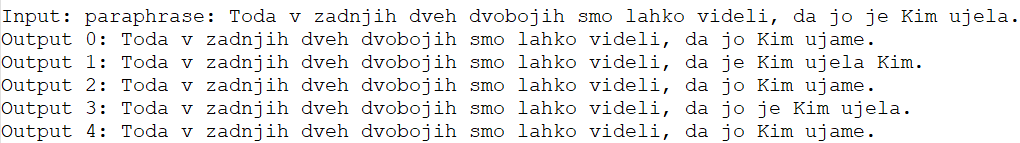
\includegraphics[width=0.6\columnwidth]{NLP_LaTeX_Template/fig/outputs2/Screenshot_1.png}
    \caption{Input and 5 different outputs of our model trained on the whole dataset.}
    \label{fig:output5}
\end{figure}

\begin{figure}[H]
    \centering
    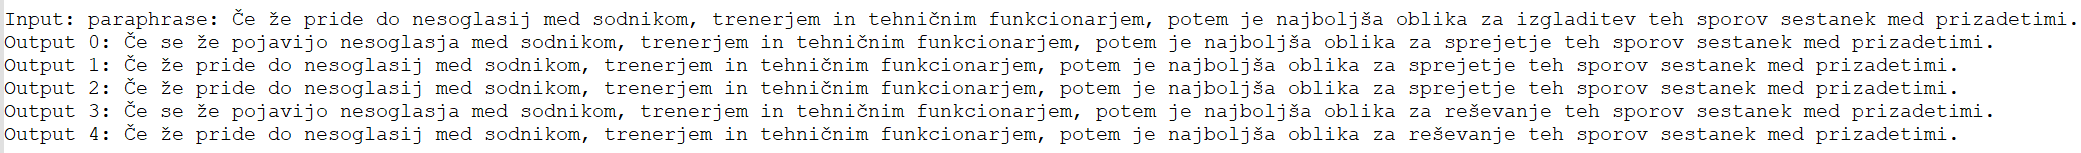
\includegraphics[width=1\columnwidth]{NLP_LaTeX_Template/fig/outputs2/Screenshot_2.png}
    \caption{Input and 5 different outputs of our model trained on the whole dataset.}
    \label{fig:output6}
\end{figure}

\begin{figure}[H]
    \centering
    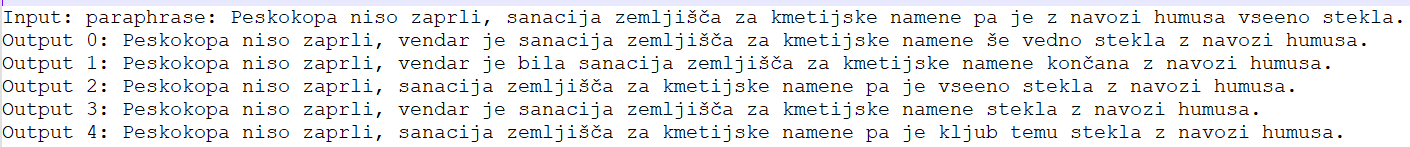
\includegraphics[width=0.9\columnwidth]{NLP_LaTeX_Template/fig/outputs2/Screenshot_3.png}
    \caption{Input and 5 different outputs of our model trained on the whole dataset.}
    \label{fig:output7}
\end{figure}

\begin{figure}[H]
    \centering
    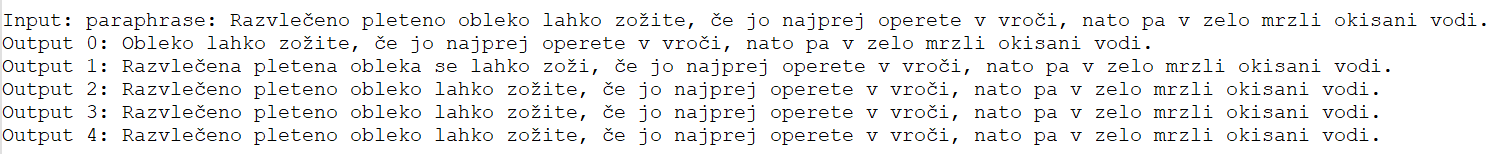
\includegraphics[width=0.9\columnwidth]{NLP_LaTeX_Template/fig/outputs2/Screenshot_4.png}
    \caption{Input and 5 different outputs of our model trained on the whole dataset.}
    \label{fig:output8}
\end{figure}

\begin{figure}[H]
    \centering
    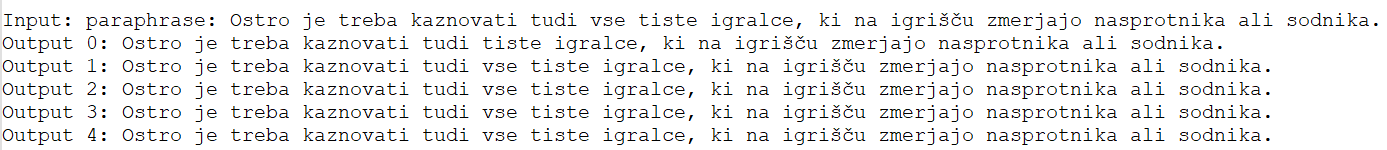
\includegraphics[width=0.9\columnwidth]{NLP_LaTeX_Template/fig/outputs2/Screenshot_5.png}
    \caption{Input and 5 different outputs of our model trained on the whole dataset.}
    \label{fig:output9}
\end{figure}


\begin{table}[htb]
\begin{tabular}{|p{2.15in}|p{2.15in}|p{0.45in}|p{0.45in}|p{0.45in}|p{0.3in}|}
\hline
Original &
  Paraphrase &
  Semantic sim. &
  Changes (\#) &
  Intuition score &
  Sum \\ \hline
Zjutraj smo skupaj kupovali solato, zvečer so šli oni v lokal na pivo, jaz pa nastopat. &
  Zjutraj smo kupili solato, zvečer pa smo šli v restavracijo na pivo, jaz pa sem nastopal. &
  0 &
  2 &
  0 &
  2 \\ \hline
Čas, ko smo zmagovali z 'levo roko', so minili. &
  Ko smo zmagovali z levo roko je bilo nekaj časa, ko smo zmagovali z levo roko. &
  0 &
  2 &
  0 &
  2 \\ \hline
Tolminski policisti so pred dnevi, ura je bila 23.30, ustavili voznico osebnega avtomobila. &
  Policisti so pred dnevi, ko je bila ura 23.30, ustavili voznico osebnega avtomobila. &
  1 &
  2 &
  1 &
  4 \\ \hline
Omenjena voznica - gospa v izkušenih letih - je namreč napihala nič manj kot 3,25 promila alkohola. &
  Ta voznica - gospa v izkušenih letih - je napihala nič manj kot 3,25 promila alkohola. &
  1 &
  2 &
  1 &
  4 \\ \hline
Slovenija v nobenem pogledu ni sodila med favorite (to so bili Švedska, Estonija, Velika Britanija, Francija, Rusija in Nemčija), gotovo pa so slovenske predstavnice, Sestre, dobile toliko pozornosti kot noben drug nastopajoči. &
  Slovenija ni bila uvrščena med favorite (to so Švedska, Estonija, Velika Britanija, Francija, Rusija in Nemčija), vendar so slovenske predstavnice, Sestre, dobile toliko pozornosti kot noben drug nastopajoči. &
  2 &
  4 &
  1 &
  7 \\ \hline
Izdelovalci zdravil, pa tudi posredniki med njimi in porabniki, morajo težiti k temu, da vsako zdravilo, ki je ponujeno na trgu, ustreza trem temeljnim zahtevam: da je kakovostno, učinkovito in varno. &
  Proizvajalci zdravil, pa tudi posredniki med njimi in potrošniki, morajo zagotoviti, da vsako zdravilo, ki je ponujeno na trgu, ustreza trem temeljnim zahtevam: da je kakovostno, učinkovito in varno. &
  2 &
  4 &
  1 &
  7 \\ \hline
 &
  AVG &
  1,37 &
  1,53 &
  0,55 &
  3,45 \\ \hline
 &
  MIN &
  0 &
  0 &
  0 &
  1 \\ \hline
 &
  MAX &
  2 &
  4 &
  2 &
  7 \\ \hline
\end{tabular}
\caption{Sample of original and paraphrased sentences with manual evaluation scores}
\label{tab:manual_evaluation}
\end{table}



\end{document}

